\documentclass[a4paper, 10pt, final, garamond]{book}
\usepackage{cours-preambule}
\graphicspath{{./figures/}}

\makeatletter
\renewcommand{\@chapapp}{Travaux pratiques -- TP}
\makeatother

% \toggletrue{student}
% \toggletrue{corrige}
% \renewcommand{\mycol}{black}
% \renewcommand{\mycol}{gray}

\hfuzz=5.003pt

\begin{document}
\setcounter{chapter}{26}

\settype{enon}
\settype{solu_prof}
\settype{solu_stud}

\chapter{\cswitch{%
	  Correction du TP
  }{%
	  Équilibre liquide/vapeur d'eau
  }%
 }

\enonce{%
	% \begin{tcn}*(exem)<ctc>"how"'t'{Capacités exigibles}
	% 	\begin{itemize}
	% 		\item Mettre en œuvre un protocole expérimental de mesure d'une grandeur
	% 		      thermodynamique énergétique
	% 	\end{itemize}
	% \end{tcn}
	% \vspace{-10pt}

	\section{Objectifs}

	\begin{itemize}
		\item Mettre en œuvre un protocole de mesure de pression et de température
		      en fonction du temps.
		\item Mesurer la pression de vapeur saturante~: grandeur caractéristique
		      d'un équilibre liquide-vapeur.
		\item Déterminer expérimentalement l'enthalpie molaire de vaporisation de
		      l'eau.
	\end{itemize}

	\section{S'approprier}
	\subsection{Pression de vapeur saturante}
	Pour un corps pur sous deux phases en équilibre thermodynamique (ici, l'eau
	sous phase liquide et gazeuse), la pression et la température ne peuvent pas
	être indépendamment fixées par l'opérataire~: la pression d'équilibre, aussi
	appelée \textbf{pression de vapeur saturante}, dépend de la température~:
	\[
		P\ind{sat}(T)
	\]
	C'est la pression du système à la température $T$ \textbf{tant que les phases
		liquide et gazeuse coexistent}.
	\subsection{Relation de \textsc{Rankine}}
	Un modèle simple conduit à considérer la relation dite de \textsc{Rankine}
	entre $P\ind{sat}$ et $T$~:
	\[
		\ln P\ind{sat} = A - \frac{B}{T}
		\qqav
		B = \frac{L_{V,m}}{R}
	\]
	avec $A$ et $B$ des constantes, $L_{V,m}$ l'enthalpie \textbf{molaire} de
	vaporisation de l'eau, et $R$ la constante du gaz parfait.
	\subsection{Dispositif expérimental}
	\begin{isd}
		\begin{itemize}
			\item On chauffe le ballon contentant de l'eau pure, \textbf{avec le robinet R
				      OUVERT}, jusqu'à ébullition. La vapeur d'eau, à pression
			      atmosphérique, envahit les canalisations.

			\item Quand on estime que le ballon est purgé de tout l'air présent
			      initialement, on ferme R et on arrête le chauffage.

			\item La température diminue alors, en même temps que la pression de la vapeur
			      qui est ici la pression de vapeur saturante tant que l'équilibre
			      diphasique se maintient.

			\item Tant que le système est à l'équilibre, on peut observer l'ébullition et il
			      existe une relation entre la pression de vapeur saturante $P\ind{sat}$
			      et la température $T$.
		\end{itemize}
		\tcblower
		\begin{center}
			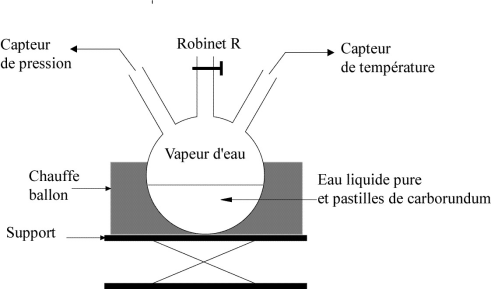
\includegraphics[width=1\linewidth]{dispo_exp}
		\end{center}
	\end{isd}
	\section{Réaliser}
	\begin{tcn}[breakable](expe)<itc>{Préparation de l'acquisition}
		\begin{enumerate}
			\item Les capteurs de pression et de température sont pré-branchés sur votre
			      carte \texttt{Arduino}. Tous les branchements sont faits. Vérifiez
			      juste la cohérence de l'affichage digital de la température et de la
			      pression.

			\item En vous connectant sur Cahier de Prépa, récupérez le fichier
			      \texttt{TP27-code\_python.py} (programme \texttt{Python} de lecture
			      des données envoyées par la carte \texttt{Arduino} à l'ordinateur) et
			      enregistrez-le dans votre espace personnel.

			\item  Ouvrez le fichier python avec \texttt{Pyzo} et exécutez-le. Si des
			      valeurs cohérentes s'affichent dans l'interpréteur, tout fonctionne~!
			      Vous êtes prêt-es pour la suite. Interrompre l'exécution avec les
			      touches \fbox{\texttt{Ctrl}} + \fbox{\texttt{I}}.
		\end{enumerate}
	\end{tcn}

	\begin{tcn}(expe)<itc>{Acquisition des valeurs}
		\begin{enumerate}[resume]
			\item Chauffer l'eau du ballon à l'aide du chauffe-ballon avec le
			      \textbf{robinet ouvert}.

			\item Quand l'eau bout depuis suffisamment longtemps pour avoir éliminé tout
			      l'air présent initialement~:
			      \begin{itemize}
				      \item fermer le robinet R en même temps que vous écartez le
				            chauffe-ballon (en abaissant le chariot élévateur)

				      \item lancez l'acquisition en exécutant le script python.
			      \end{itemize}

			\item Arrêter l'enregistrement quand la pression stagne (aux environs de
			      \SIrange{0.2}{0.3}{bar}). Si la pression remonte au cours de
			      l'expérience, c'est un problème d'étanchéité, les données postérieures
			      à cette augmentation de pression ne seront pas exploitables.
		\end{enumerate}
	\end{tcn}
	\begin{tcn}*[](prop)"bomb"{Attention}
		Si vous devez recommencer votre expérience et que vous devez remettre le
		chauffe-ballon en route, \textbf{pensez à rouvrir le robinet}~! Sinon, la
		pression va fortement augmenter et c'est le risque d'explosion, de brûlure, et
		de divers dégâts physiques permanents.
	\end{tcn}
}%

\setcounter{section}{3}
\section{Analyser et conclure}
\enonce{%
	Ouvrir \texttt{Regressi} et ouvrir le fichier \texttt{data\_arduino.txt} dans
	le dossier \texttt{document} de votre espace personnel (sélectionner le type
	\texttt{txt} dans le menu déroulant). Vérifier que vous avez 3 colonnes de
	données~: temps $t$, température $T$ et pression $P$.
}%

\setlist[blocQR,1]{label=\sqenumi}
\QR{%
	Afficher en superposition sur le même graphe $P$ et $T$ en fonction du temps.
	Prendre soin de choisir une échelle à gauche pour $P$ et une échelle à droite
	pour $T$. Décocher l'option \texttt{zéro inclus}. Imprimer.
}{%
	solu
}%
\QR{%
	Créer les variables nécessaires à la détermination des coefficients du modèle
	de \textsc{Rankine}, et vérifier que vos données soient modélisables par une
	régression linéaire bien choisie. Rédiger quelle est la régression et les
	valeurs des paramètres obtenus sur votre copie.
}{%
	solu
}%
\QR{%
	Les données tabulées donnent $\ell_V = \SI{2257}{kJ.kg^{-1}}$ pour l'enthalpie
	\textbf{massique} de vaporisation. Comparer à la valeur que vous avez obtenue
	par régression. On rappelle la masse molaire de l'eau~: $M =
		\SI{18}{g.mol^{-1}}$.
}{%
	solu
}%

\end{document}
